%% abtex2-modelo-trabalho-academico.tex, v-1.9.7 laurocesar
%% Copyright 2012-2018 by abnTeX2 group at http://www.abntex.net.br/ 
%%
%% This work may be distributed and/or modified under the
%% conditions of the LaTeX Project Public License, either version 1.3
%% of this license or (at your option) any later version.
%% The latest version of this license is in
%%   http://www.latex-project.org/lppl.txt
%% and version 1.3 or later is part of all distributions of LaTeX
%% version 2005/12/01 or later.
%%
%% This work has the LPPL maintenance status `maintained'.
%% 
%% The Current Maintainer of this work is the abnTeX2 team, led
%% by Lauro César Araujo. Further information are available on 
%% http://www.abntex.net.br/
%%
%% This work consists of the files abntex2-modelo-trabalho-academico.tex,
%% abntex2-modelo-include-comandos and abntex2-modelo-references.bib
%%

% ------------------------------------------------------------------------
% ------------------------------------------------------------------------
% abnTeX2: Modelo de Trabalho Academico (tese de doutorado, dissertacao de
% mestrado e trabalhos monograficos em geral) em conformidade com 
% ABNT NBR 14724:2011: Informacao e documentacao - Trabalhos academicos -
% Apresentacao
% ------------------------------------------------------------------------
% ------------------------------------------------------------------------

\documentclass[
	% -- opções da classe memoir --
	12pt,				% tamanho da fonte
	%openright,			% capítulos começam em pág ímpar (insere página vazia caso preciso)
	oneside,			% para impressão em recto e verso. Oposto a oneside
	a4paper,			% tamanho do papel. 
	% -- opções da classe abntex2 --
	%chapter=TITLE,		% títulos de capítulos convertidos em letras maiúsculas
	%section=TITLE,		% títulos de seções convertidos em letras maiúsculas
	%subsection=TITLE,	% títulos de subseções convertidos em letras maiúsculas
	%subsubsection=TITLE,% títulos de subsubseções convertidos em letras maiúsculas
	% -- opções do pacote babel --
	english,			% idioma adicional para hifenização
	brazil				% o último idioma é o principal do documento
	]{abntex2}
% ---
% Pacotes básicos 
% ---
\usepackage{lmodern}			% Usa a fonte Latin Modern			
\usepackage[T1]{fontenc}		% Selecao de codigos de fonte.
\usepackage[utf8]{inputenc}		% Codificacao do documento (conversão automática dos acentos)
\usepackage{indentfirst}		% Indenta o primeiro parágrafo de cada seção.
\usepackage{color}				% Controle das cores
\usepackage{graphicx}			% Inclusão de gráficos
\usepackage{microtype} 			% para melhorias de justificação
% ---
		
% ---
% Pacotes adicionais, usados apenas no âmbito do Modelo Canônico do abnteX2
% ---
\usepackage{lipsum}				% para geração de dummy text
% ---

% ---
% Pacotes de citações
% ---
\usepackage[brazilian,hyperpageref]{backref}	 % Paginas com as citações na bibl
\usepackage[alf]{abntex2cite}	% Citações padrão ABNT

\usepackage{caption}

% --- 
% CONFIGURAÇÕES DE PACOTES
% --- 

% ---
% Configurações do pacote backref
% Usado sem a opção hyperpageref de backref
\renewcommand{\backrefpagesname}{Citado na(s) página(s):~}
% Texto padrão antes do número das páginas
\renewcommand{\backref}{}
% Define os textos da citação
\renewcommand*{\backrefalt}[4]{
	\ifcase #1 %
		Nenhuma citação no texto.%
	\or
		Citado na página #2.%
	\else
		Citado #1 vezes nas páginas #2.%
	\fi}%
% ---

% ---
% Informações de dados para CAPA e FOLHA DE ROSTO
% ---
\titulo{Previsão de carga de curto prazo \\ utilizando técnicas de redes neurais artificiais}
\autor{Daniel Cezar Salgado}
\local{Itajubá, Brasil}
\data{2019}
\orientador{Camila Paes Salomon}
\coorientador{Hanneli Carolina Andreazzi Tavante}
\instituicao{%
  Universidade Federal de Itajubá -- UNIFEI
  \par
  Instituto de Sistemas Elétricos e Energia -- ISEE}
\tipotrabalho{Tese (Graduação)}
% O preambulo deve conter o tipo do trabalho, o objetivo, 
% o nome da instituição e a área de concentração 
\preambulo{Monografia apresentada ao Instituto de Sistemas Elétricos e Energia, da Universidade Federal de Itajubá, como parte dos requisitos para obtenção do título de Engenheiro Eletricista.}
% ---


% ---
% Configurações de aparência do PDF final

% alterando o aspecto da cor azul
\definecolor{blue}{RGB}{41,5,195}

% informações do PDF
\makeatletter
\hypersetup{
     	%backref=true,
		pdftitle={\@title}, 
		pdfauthor={\@author},
    	pdfsubject={\imprimirpreambulo},
	    pdfcreator={LaTeX with abnTeX2},
		pdfkeywords={abnt}{latex}{abntex}{abntex2}{trabalho acadêmico}, 
		colorlinks=true,       		% false: boxed links; true: colored links
    	linkcolor=blue,          	% color of internal links
    	citecolor=black,        		% color of links to bibliography
    	filecolor=magenta,      		% color of file links
		urlcolor=blue,
		bookmarksdepth=4
}
\makeatother
% --- 

% ---
% Posiciona figuras e tabelas no topo da página quando adicionadas sozinhas
% em um página em branco. Ver https://github.com/abntex/abntex2/issues/170
\makeatletter
\setlength{\@fptop}{5pt} % Set distance from top of page to first float
\makeatother
% ---

% ---
% Possibilita criação de Quadros e Lista de quadros.
% Ver https://github.com/abntex/abntex2/issues/176
%
\newcommand{\quadroname}{Quadro}
\newcommand{\listofquadrosname}{Lista de quadros}

\newfloat[chapter]{quadro}{loq}{\quadroname}
\newlistof{listofquadros}{loq}{\listofquadrosname}
\newlistentry{quadro}{loq}{0}

% configurações para atender às regras da ABNT
\setfloatadjustment{quadro}{\centering}
\counterwithout{quadro}{chapter}
\renewcommand{\cftquadroname}{\quadroname\space} 
\renewcommand*{\cftquadroaftersnum}{\hfill--\hfill}

\setfloatlocations{quadro}{hbtp} % Ver https://github.com/abntex/abntex2/issues/176
% ---

% --- 
% Espaçamentos entre linhas e parágrafos 
% --- 

% O tamanho do parágrafo é dado por:
\setlength{\parindent}{1.3cm}

% Controle do espaçamento entre um parágrafo e outro:
\setlength{\parskip}{0.2cm}  % tente também \onelineskip

% ---
% compila o indice
% ---
\makeindex
% ---

% ----
% Início do documento
% ----
\begin{document}

% Seleciona o idioma do documento (conforme pacotes do babel)
%\selectlanguage{english}
\selectlanguage{brazil}

% Retira espaço extra obsoleto entre as frases.
\frenchspacing 

% ----------------------------------------------------------
% ELEMENTOS PRÉ-TEXTUAIS
% ----------------------------------------------------------
% \pretextual

% ---
% Capa
% ---
\imprimircapa
% ---

% ---
% Folha de rosto
% (o * indica que haverá a ficha bibliográfica)
% ---
%\imprimirfolhaderosto*
% ---

% ---
% Inserir folha de aprovação
% ---

% Isto é um exemplo de Folha de aprovação, elemento obrigatório da NBR
% 14724/2011 (seção 4.2.1.3). Você pode utilizar este modelo até a aprovação
% do trabalho. Após isso, substitua todo o conteúdo deste arquivo por uma
% imagem da página assinada pela banca com o comando abaixo:
%
% \begin{folhadeaprovacao}
% \includepdf{folhadeaprovacao_final.pdf}
% \end{folhadeaprovacao}
%
\begin{folhadeaprovacao}

  \begin{center}
    {\ABNTEXchapterfont\large\imprimirautor}

    \vspace*{\fill}\vspace*{\fill}
    \begin{center}
      \ABNTEXchapterfont\bfseries\Large\imprimirtitulo
    \end{center}
    \vspace*{\fill}
    
    \hspace{.45\textwidth}
    \begin{minipage}{.5\textwidth}
        \imprimirpreambulo
    \end{minipage}%
    \vspace*{\fill}
   \end{center}

   \assinatura{\textbf{\imprimirorientador} \\ Orientadora} 
   \assinatura{\textbf{\imprimircoorientador} \\ Coorientadora}
   \assinatura{Convidado}
   %\assinatura{\textbf{Professor} \\ Convidado 3}
   %\assinatura{\textbf{Professor} \\ Convidado 4}
      
   \begin{center}
    \vspace*{0.5cm}
    {\large\imprimirlocal}
    \par
    {\large\imprimirdata}
    \vspace*{1cm}
  \end{center}
  
\end{folhadeaprovacao}
% ---

% ---
% Agradecimentos
% ---
\begin{agradecimentos}

	Agradeço às minhas orientadoras, Camila Salomon e Hanneli Tavante, por toda a orientação e disponibilidade para me ajudar em todos os momentos de dúvidas.
	Ao meu irmão pelo exemplo e inspiração.
	Aos meus pais por me ensinarem todos valores importantes que eu carrego comigo por toda minha vida e por todo seu amor. 
	
\end{agradecimentos}
% ---

% ---
% Dedicatória
% ---
\begin{dedicatoria}
   \vspace*{\fill}
   \centering
   \noindent
   \textit{	Dedico esse trabalho à minha família, sempre presentes com amor incondicional e apoiadores de todas as minhas decisões e às minhas orientadoras, por toda a paciência para me guiar nesse trabalho e na minha evolução acadêmica.	}  \vspace* {\fill}
\end{dedicatoria}
% ---

% ---
% RESUMOS
% ---

% resumo em português
\setlength{\absparsep}{18pt} % ajusta o espaçamento dos parágrafos do resumo
\begin{resumo}
	O sistema elétrico depende de grandezas instantâneas para seu adequado funcionamento com valores operativos dentro das faixas específicas para entregar energia aos consumidores e manter os equipamentos que o operam em valores seguros. Para isso, é feito um planejamento em diferentes horizontes para que o sistema continue operando e consiga suprir todas as demandas de carga que possam ocorrer. Uma das etapas é a previsão de carga elétrica que deverá ser suprida. A previsão de carga de curto prazo, dentre alguns minutos até 1 dia antes da operação, é utilizada para monitoramento e determinação da estabilidade para diferentes pontos quando houver a ocorrência de eventos inesperados como faltas ou mudanças climáticas que façam a proteção do sistema atuar e modificar a sua dinâmica. 
	Novas tecnologias têm sido adotadas para melhorar a utilização de recursos do sistema, tal que formem uma grande rede com maior monitoramento e controle. Redes inteligente utilizam de medidores residenciais com taxas de amostragem muito maiores que os tradicionais, e necessitam de uma infraestrutura muito mais complexa para o correto armazenamento e posterior utilização dos dados gerados. Técnicas de aprendizagem profunda são capazes de analisar grande volume de dados em tempos factíveis e podem aprender a fazer previsões quando treinadas com dados passados. 
	
	\textit{Long-short term memory} (LSTM) é um modelo de rede neural recorrente que é capaz de analisar dados sequenciais e gerar novas sequencias de dados, tais como em modelos preditivos. Na sua estrutura, ele mantêm a referência temporal e a importância da sequência, o que pode ser um benefício para a utilização do sistema elétrico com previsões de curto prazo. 
	A base de dados do órgão Irlandês CER, com medidas de mais de 5000 residências e pequenos e médios empreendimentos com medições com frequência de 30 minutos durante 1 ano e meio é utilizado para a validação da proposta, com a limpeza e organização dos dados e rede neural LSTM sendo empregado diversas tecnologias utilizadas no mercado para desenvolvimento de modelos de aprendizagem profunda, tais como linguagem Python, Tensorflow, Keras, Pandas e Colab. 
		
	\vspace{\onelineskip}
 
	\textbf{Palavras-chave}: Aprendizagem Profunda, Redes Neurais Recorrentes, LSTM, Previsão de Carga, Redes Inteligentes, Python, Tensorflow, Keras.
	
	
	
	% Deixar clara a proposta do trabalho "O objetivo deste trabalho é fazer a previsao de carga utilizando LSTM ... é validado com a base de dados..."
\end{resumo}

% resumo em inglês
\begin{resumo}[Abstract]
 \begin{otherlanguage*}{english}
  The electric grid relies on instantaneous measurements for its adequate operation, with operating values within specific ranges to deliver power to costumers and maintain the equipments which operate safe. For this, a plan is made for different horizons so that the system keeps operating and able to supply all loads which might happen. One of the steps is the load forecasting. Short term load forecasting, within minutes to a day before the operation, is used to monitoring and establishing system stability in different points when some unexpected event occur, like faults or sudden climatic changes that make the protection devices trip and modify the system dynamics. 
   New technologies have been used to enhance system resources use, such that build a big interconnected network with improved monitoring and controlling. Smart grids makes use of residential load meter with much higher sampling rates than the traditional, and need a much more complex infrastructure for the appropriate storage and further use of the generated data. Deep learning techniques are capable of analysing large amounts of data in feasible time and can learn to forecast when trained with past data. 
   
   Long-short term memory (LSTM) is a model of recurrent neural network that is capable of analyse sequential data and generate new sequences, as forecasting models. In its structure, it keeps the time reference and the significance of the sequence, what can be an advantage to using it for short term load forecast. 
   The database of Irish comission CER, with more than 5000 residential and small and medium enterprises load measurements with sampling rate of 30 minutes during 1 and half year is used to validate the proposal, with data cleaning and conditioning and neural network LSTM used alongside other technologies very spread in the development market as Python, Tensorflow, Keras, Pandas e Colab. 

   \vspace{\onelineskip}
 
   \noindent 
   \textbf{Keywords}: Deep Learning, Recurrent Neural Networks, LSTM, Load Forecast, Smart Grids, Python, Tensorflow, Keras.
 \end{otherlanguage*}
\end{resumo}


% ---
% inserir lista de ilustrações
%% ---
\pdfbookmark[0]{\listfigurename}{lof}
\listoffigures*
\cleardoublepage
% ---

% ---
% inserir lista de quadros
% ---
%\pdfbookmark[0]{\listofquadrosname}{loq}
%\listofquadros*
%\cleardoublepage
% ---

% ---
% inserir lista de tabelas
% ---
\pdfbookmark[0]{\listtablename}{lot}
\listoftables*
\cleardoublepage
% ---

% ---
% inserir lista de abreviaturas e siglas
% ---
\begin{siglas}
	\item[AI] Inteligência Artificial \textit{(Artificial Intelligence)}
	\item[API] Interface de Programação de Aplicação \textit{(Application Programming Inferface)}
	\item[CE] \textit{Commission for Energy Regulation }
	\item[DL] Aprendizagem Profunda \textit{(Deep Leaning)}
	\item[DNN] Redes Neurais Profundas \textit{(Deep Neural Networks)}
	\item[LSTM] \textit{Long-Short Term Memory}
	\item[ML] Aprendizado de Máquina \textit{(Machine Learning)}
	\item[MLP]  \textit{Multi-layer Perceptron}
	\item[RNN] Redes Neurais Recorrentes \textit{(Recurrent Neural Networks)}
\end{siglas}
% ---

% ---
% inserir lista de símbolos
%% ---
%\begin{simbolos}
%  \item[$ \alpha $] Passo de treinamento
%  \item[$ \Lambda $] Lambda
%%  \item[$ \zeta $] Letra grega minúscula zeta
%%  \item[$ \in $] Pertence
%\end{simbolos}
% ---

% ---
% inserir o sumario
% ---
\pdfbookmark[0]{\contentsname}{toc}
\tableofcontents*
\clearpage
%\cleardoublepage
% ---



% ----------------------------------------------------------
% ELEMENTOS TEXTUAIS
% ----------------------------------------------------------
\textual

% ----------------------------------------------------------
% Introdução (exemplo de capítulo sem numeração, mas presente no Sumário)
% ----------------------------------------------------------
\chapter{Introdução}
% ----------------------------------------------------------
	O sistema elétrico é uma rede complexa e interligada em diferentes pontos com barras geradoras de energia, linhas de transmissão levando energia gerada até as barras de consumidores, e cargas que utilizarão essa energia, tal que toda a quantidade produzida deve ser consumida ou é naturalmente perdida ao longo das linhas ou nos equipamentos. Gerir de forma otimizada os recursos existentes é uma tarefa que pode determinar o sucesso ou fracasso de um empreendimento quando suas fontes são limitadas, como reservatórios de represas e reservas de carvão e gás, e também determina o seu custo. Conhecer a demanda dos recursos pode ajudar no planejamento financeiro de acordo com as necessidades, e com o retorno sobre o investimento desejado, podendo utilizar da geração e transmissão de energia mais caras ou mais mais baratas. 
	Sistemas de armazenamento de energia elétrica ainda são tecnologias de elevado custo e portanto não são largamente utilizadas para suprir grandes blocos de energia. Assim, deve sempre haver um balanço entre a energia gerada e consumida, e perdas longo do sistema, que quando desproporcionais podem levar a alteração dos valores de tensão nas barras do sistema, retirando-os da faixa aceitável ou deixar o sistema mais susceptíveis a pequenas falhas em equipamento e linhas. 
	
	% ------> Referência
	
	É importante, então, uma estimativa satisfatória da carga a ser consumida, para que possa determinar a quantidade de energia a ser gerada e quais as usinas geradoras que podem suprir essa necessidade conhecendo o sistema físico e possuir modelos adequados para representá-lo sabendo a capacidade e limites de cada componente que o compõem. Previsão do comportamento, tendências e variações das cargas ligadas no sistema ao longo do tempo auxilia na tomada de decisão quanto ao planejamento e operação do sistema. 	
	
	Nas concessionárias de distribuição, é interessante ter a previsão de cargas da sua concessão para o planejamento das transações de compra da energia que ela revenderá. Com isso, podem otimizar os fornecedores, seus preços e a quantidade de energia necessária, minimizando seus gastos em diferentes horários do dia com diferentes tarifas \cite{ReviewSmartMeterLoadForecastingTechniques}. 
	
	% ------> Monitoramento + Smart Grid + facilitar tomada de decisão

	A geração de energia elétrica é historicamente feita por grandes usinas que geram um grande bloco de energia elétrica tal que ele é transmitido até chegar a carga para ser consumida. Novas fontes de energia, como eólica e solar, e novas tecnologias, como armazenadores de energia e até carros elétricos, permitem que a geração possa ser realizada localmente em menor escala e de forma distribuída já na distribuição e traz novos desafios para a modelagem, planejamento e operação do sistema. Isso torna as cargas mais voláteis, mudando a característica de consumo e utilização de redes de transmissão e distribuição, tal que a geração e consumo de consumidores individuais tendem a ser mais difíceis de se prever. Quando se modelam as cargas como blocos agregados, com o consumo direto da subestação, o seu comportamento segue um padrão. Já quando se modelam cargas individuais, o padrão de consumo depende da característica comportamental humana e de seus costumes em cada residência, o que é muito variado. \cite{kong2017short}		
	
	Em um esforço para melhorar a utilização do sistema elétrico, em especial na transmissão e distribuição, novas tecnologias têm sido adotadas e utilizadas em equipamentos que tornem o sistema mais conectado e confiável. Sistemas de comunicação são inseridos nos dispositivos que compõem o sistema, tal que forme uma rede interligada e inteligente, capaz não só de trocar informação entre eles, como também armazenar dados e processá-los. As redes inteligentes utilizam sensores e medidores em todos as partes do sistema, desde geração até o consumidor final na distribuição e carga, podendo até mesmo serem consideradas em eletrodomésticos em cenários mais específico, abrindo possibilidades de supervisão e controle em uma escala como nunca houve. 
	
	Para minimizar desperdícios e perdas no sistema elétrico e tornar a geração e distribuição mais eficientes, redes inteligentes têm sido a aposta para maior flexibilidade e controle. Para isso, ela tem que ser capaz de se adaptar a mudanças na demanda e distribuir eficientemente a geração para diferentes fontes distribuídas e renováveis \cite{choueiki1997building}. Dessa forma, a previsão de cargas tanto agregadas nos alimentadores e nas subestações como também nos consumidores finais tem papel muito importante.
	
	Medidores inteligentes de energia elétrica possuem mais funcionalidades que medidores tradicionais. Com eles é possível medir o consumo de energia remotamente através de uma rede de comunicação bidirecional e direta entre consumidores e concessionárias, e com uma frequência que pode chegar até a alguns minutos \cite{trials2008findings}, o que cria uma base de dados muito maior das que se tem tradicionalmente. A implementação desses medidores é um passo fundamental para a estrutura de redes inteligentes que está em construção em todo o mundo e diferentes iniciativas estão sendo construídas para se estudar a adoção de tais tecnologias.
	
	Em 2007, o órgão Commission for Energy Regulation (CER), responsável por supervisionar as legislações de energia elétrica e gás da Irlanda, lançou um projeto piloto de tecnologia de medidores inteligentes de energia elétrica para melhorar seu entendimento das necessidades para o desenvolvimento de medidores inteligentes em parceria com as distribuidoras de energia elétrica do país. \cite{trials2008findings} Com esse projeto, CER tinha como objetivo validar seus projetos de infraestrutura de tecnologia da informação necessária, tais como comunicação, hardware e softwares; quantificar possíveis problemas e riscos que poderiam surgir com a tecnologia em programas nacionais; adquirir conhecimento de negócios para um projeto de tal dimensão, tais como novos modelos de tarifas e comportamento no consumo dos seus consumidores; e ainda analisar o custo-benefício de tal empreendimento. Durante os testes, foram realizadas medições em 6700 residências e pequenas e médias empresas, tais que fossem representativas do país, a cada 30 minutos por um período de 18 meses entre julho de 2009 e dezembro de 2010. Apos as medições e relatórios, os dados foram disponibilizados para fins de testes e pesquisas, e utilizado nesse trabalho.	
	
	Cada vez mais dados são gerados e armazenados, extrapolando a capacidade de processamento de toda base de  dados através de modelos matemáticos e estatísticos já consolidados. Ciência de dados não se trata de uma disciplina nova, mas de técnicas que já são utilizadas para fornecer conclusões a partir da análise de dados. Por outro lado também só são úteis quando se consegue agregar valor a eles, podendo até gerar outros dados como resultado.  A capacidade de armazenamento, processamento e comunicação tem crescido rapidamente nos últimos anos, gerando grandes bases de dados que necessitam de novas técnicas para serem adequadamente utilizada, surge então o termo "\textit{Big data}", quando o tamanho de tal base de dados também se torna parte do problema. \cite{loukides2011data} Técnicas de inteligência artificial são utilizadas para se analisar essas bases de dados, utilizando de Redes Neurais Profundas (DNN, do inglês \textit{Deep Neural Networks}).
	
	Novas técnicas de Aprendizagem Profunda (DL, do inglês \textit{Deep Learning}) constituem de arquiteturas de DNN que permitem aprendizado de relações complexas entre entradas e saídas identificam padrões em grande base de dados e podem agregar valor a eles, gerando novos resultados \cite{amarasinghe2017deep}. Utilizam de arquiteturas com múltiplas camadas para extração de características e reconhecimentos de padrões nos dados podendo descobrir grandes estruturas nos dados.

\section{Previsão de cargas e horizontes}
	
	O ser humano em sua história sempre tentou identificar padrões em eventos para prever como eles ocorrerão no futuro, seja em elementos simples como estações do ano para plantações, e também em mais complexas, como para o mercado financeiro. Para isso, é preciso olhar para o passado e assumir que os eventos ocorrerão novamente com determinada frequência, tal que os padrões sejam identificados e seja possível saber como eles ocorrerão no futuro.  Quaisquer que sejam as circunstâncias e o horizonte, previsão sempre pode fornecer um suporte ao planejamento mais eficiente.
	
	Séries temporais são séries de dados que representam uma sequência de eventos igualmente intervalados com o passar do tempo. Assim, analisando os dados passados, pode-se criar estimativas de como os eventos ocorrerão no futuro. Essas séries podem ser decompostas em alguns elementos como tendências, locais ou globais de crescimento ou decrescimento; ciclos sazonais, como os dados se comportam em determinados períodos; pulsos ou passos, com mudanças drásticas ao redor do seu valor original para assumir um novo patamar. Para cada domínio, diferentes parâmetros precisam ser analisados. Por exemplo, para a previsão de energia elétrica, sabe-se que a temperatura, época do ano e economia são fatores que determinam o comportamento das cargas. Previsões irão responder a determinada pergunta, tal como qual será o consumo da carga nos próximos dias da semana. 
	
	Modelos preditivos podem ser feitos de muitas formas, tal que cada uma oferece suas vantagens e desvantagens com suas particularidades e funcionam melhor com diferentes horizontes de previsão. São o período de tempo para cada previsão que podem ser de longo, médio ou curto prazo, cada uma com diferentes utilidades para o planejamento, gerenciamento e operação de cada parte do sistema. Podem ainda ter diferentes escalas de tempo ou ser desde o consumidor final até todo o sistema elétrico. \cite{ReviewSmartMeterLoadForecastingTechniques}
	
	%Operação do sistema - confiabilidade em níveis aceitáveis mas com custos mínimos  - diferentes horizontes

	% ----------> Referências daqui pra baixo	
	
	% Horizonte de longo prazo
	O planejamento e desenvolvimento de cada parte do sistema, em especial do sistema de transmissão de energia elétrica, requer simulações e previsões de carga e geração em diferentes cenários. Envolvem inúmeras fontes de dados de diferentes domínios, tais que todas são geradas por outras previsões, dessa forma as incertezas e riscos das medidas e modelos se propagam ao longo de cada etapa e tendem a aumentar. 
	
	Essa previsão com horizonte de décadas a frente é utilizada para expansão e crescimento do sistema, maximizando lucros, segurança e confiabilidade. Modificações do sistema elétrico envolvem elevados custos, e necessitam de tempo longo para que sejam implementadas, tais como construção de novas usinas, subestações e linhas de transmissão, licenças ambientais, compras de equipamentos, entre outros, e requerem planejamentos de obras civis e financeiro para serem realizadas.  	
	Dessa forma, é mais importante saber o que será necessário do que quando, então data e horário não são tão importantes quanto a localização e capacidade. 	
	
	% Horizonte de médio prazo	
	O sistema elétrico é uma rede de componentes que deve funcionar intermitentemente, sem a possibilidade de parada de fornecimento de energia para o consumidor e para isso rotas e conexões alternativas são possíveis em um sistema malhado. Mas concomitantemente, equipamentos necessitam de paradas temporárias para manutenção, uma vez que possuem grande valor financeiro e requerem cuidados adequados para seu correto funcionamento e manterem sua vida útil prolongada e manter a prevenção de falhas e possíveis interrupções no fornecimento. Mas isso só é possível com um calendário adequado de paradas e pode-se criar esse calendário com base na previsão de cargas que o sistema precisará suprir e ainda minimizar os custos de manutenção, em horários e com recursos necessários. 
	
	Previsão de médio prazo está relacionada com o planejamento de operações do sistema elétrico, criando diferentes cenários de operação com diferentes estratégias de operação e contenção para cada. Melhorias na infraestrutura e novos componentes e conexões no sistema são possíveis em menor escala. Com horizonte de alguns meses até o dia anterior da operação, as previsões auxiliam na tomada de decisão para melhor utilização de equipamentos e estrutura do sistema, otimizando sua performance e maximizando o retorno sobre o investimento feito sobre eles. 
	
	% Horizonte de curto prazo
	Na operação do sistema, o fornecimento de energia deve se manter constante para que tudo solicitado pelas cargas seja atendido. Na ocorrência de uma falta e atuação do sistema de proteção na sua contenção, devem-se adotar medidas para reorganizar a configuração do sistema mantendo todas as cargas. No horizonte de curto prazo, previsões até uma hora antes do momento da operação podem ajudar na correta manutenção da estabilidade e confiabilidade do sistema elétrico. Nesse horizonte pode-se realizar pequenas modificações na sua infraestrutura, tais como melhorias, reparos e condicionamento de equipamentos de monitoramento e proteção. É um horizonte para as ações praticamente instantâneas durante o período da operação do planejamento e estratégias realizadas até o dia anterior a fim de minimizar riscos durante a operação. 
	
	Em casos mais severos,  com mudanças inesperadas das condições climáticas ou faltas e falhas, no qual ocorra também uma mudança inesperada das cargas ligadas no sistema, podem-se realizar novas previsões dentro do mesmo dia para análise de contingência, estimando como será a variação da carga já presente e determinar como será o religamento dos equipamentos e das cargas que foram rejeitadas pela proteção. E ainda novas ações preventivas podem ser tomadas, manutenções podem ser canceladas e novas faltas contidas, evitando maiores indisponibilidades do fornecimento de energia. 
	
	A crescente quantidade de dados sendo coletada e armazenada é um desafio para modelos preditivos estatísticos visto que não é possível processar todos em tempo factível, principalmente em previsões de curto prazo que necessitam de tempos de processamento mais velozes. Técnicas de DL auxiliam essa análise e podem identificar padrões que não seriam possíveis encontrar de outra forma. 
	
%	Consumidores podem otimizar a utilização de seus equipamentos elétricos em diferentes horários para diferentes tarifas.  

	Dessa forma, a precisão das previsões de carga tem impacto significante nas operações do sistema elétrico. Sabe-se que subestimar a demanda de carga por acarretar na compra de energia mais cara do mercado no momento da operação, e sobrestimar pode fazer com que unidade geradoras sejam partidas ou paradas sem real necessidade, o que também acarreta em maiores custos operacionais \cite{choueiki1997building}. É possível, também, ter-se um controle e monitoramento mais detalhado em redes de distribuição a nível de consumidores finais, tal que na ocorrência de faltas possa redirecionar o fluxo de carga por caminhos alternativos criados com chaveamentos para novos arranjos, reestabelecendo a maior quantidade de consumidores possíveis. Assim, modelos confiáveis e com baixos erros de previsão de cargas são de grande importância e utilidade.	
	
	\section{Técnicas utilizadas para previsão de cargas}

	Previsão de cargas no sistema elétrico é um recurso já utilizado pelas distribuidoras em suas concessões para auxiliar na sua gestão de recursos e compras no mercado de energia elétrica. Novas técnicas que utilizam de aprendizado de máquina tem sido propostas e utilizadas. Autoencoders, redes neurais recorrentes, LSTM, redes neurais convolucionais, máquinas de Boltzmann restritas e profundas e \textit{Deep Belief Networks} apresentam bons resultados com baixos erros e se combinadas podem apresentar ainda melhores resultados. \cite{almalaq2017review} 
	
	Para a previsão de curto prazo, o modelo auto-regressivo integrado de médias móveis (ARIMA, do inglês Autoregressive integrated moving average) é vastamente utilizado, como em \cite{fan1994real}.	Redes de perceptron em multicamada (MLP, do inglês \textit{Multilayer Perceptron}) apresentam resultados satisatórios, com pequenos erros para a previsão de cargas de curto prazo, como mostrados em \cite{yalcinoz2005short} e \cite{ho1992short}.
	
	Com o objetivo de aprimorar a operação do sistema de energia elétrico dos Estados Unidos, a Electric Power Reseach Institure (EPRI), financiou a Southern Methodist University e \textit{PRT, Inc} para o desenvolvimento conjunto de um programa computacional para previsão de cargas horárias. \textit{Artificial Neural Network Short-Term Load Forecaster} (ANNSTLF) é uma rede neural artificial para previsão de carga horária do sistema elétrico que permite identificar correlações entre parâmetros de entrada como carga elétrica, condições climáticas (como temperatura e umidade relativa), dia da semana e do ano, horário do dia em séries temporais. Também utiliza um parâmetro para feriados e dias especiais, um vez que se sabe que a carga pode variar da série histórica em determinados dias e como eles aparecem com pouca frequência, uma vez por ano, a rede não consegue se adaptar adequadamente e os erros se tornam elevados. \cite{khotanzad1998annstlf}

	Para o treinamento adequado do programa desenvolvido, 2 a 3 anos de dados históricos de todas as variáveis de entrada são necessários, utilizando de um conjunto de treinamento cruzado (\textit{Cross Validation Set}) para evitar sobretreinamento (\textit{overtraining}), e é possível predizer a condição de carga horária para os 35 dias seguintes, sendo atualizada com o passar do tempo se forem fornecidos os dados a cada hora. Diferentemente do que é proposto nesse trabalho, a arquitetura da rede neural implementada é baseada em Feedforward Perceptron Multicamada e foi escolhida por não ser de grande complexidade comparada com outras como redes neurais recorrentes (RNN, do inglês \textit{Recurrent Neural Networks}) e essas não terem apresentado maiores vantagens em seus testes.


% Como é feito o treinamento: -----------------------------------------------
% To avoid over-training, the cross-validation method is used. The training set is divided into two sets. For instance, if three years of data is available, it is divided into a two-year and a one-year set. The first set is used to train the MLP and the second set is used to test the trained model after every few hundred passes over the training data. The error on the validation set is examined. Typically this error decreases as the number of passes over the training set is increased until the ANN is over-trained, as signified by a rise in this error. Therefore, the training is stopped when the error on the validation set starts to increase. This procedure yields the appropriate number of epochs over the training set. The entire three years of data is then used to re-train the MLP using this number of epochs.
% ----------------------------------------------------------
	
	Cargas individuais apresentam outros obstáculos para suas previsões, uma vez que a base de dados tende a se tornar cada vez maior e o processamento deixa de ser realizado em  um tempo factível. Em outros domínios, técnicas de aprendizagem profunda são utilizados com alternativa para superar tais dificuldades.

	\section{Proposta do trabalho}
	
	Nesse trabalho é proposta a previsão de cargas de curto prazo utilizando um modelo de RNN, \textit{Long-short Term Memory} (LSTM), através de treinamento com dados sequenciais de medidas de consumo elétrico. Para avaliação dos resultados será utilizado uma parte da base de dados irlandesa fornecida pelo CER, diferente da base de treinamento, para teste e avaliação dos erros da saída obtida comparadas com as saídas esperadas. No capítulo 2, serão apresentados os modelos de inteligência artificial, aprendizado de máquina e redes neurais utilizados. No capítulo 3, serão apresentadas as ferramentas utilizadas para as simulações e avaliações dos resultados. No capítulo 4, é apresentada a modelagem teórica proposta, da limpeza e condicionamento da base de dados e posteriores resultados de testes preliminares. No capítulo 5, será apresentado a modelagem da rede neural com melhores desempenhos e seu resultado. O capítulo 6 conclui o trabalho proposto.
	
\chapter{Fundamentação Teórica}

%	Dificuldade de Redes Neurais: Determinar a complexidade apropriada da rede
%	Evitar overfitting
%		model selection: escolher a quantidade de camadas ocultas - método prunning
%		Regularização - Weight decay e adição de ruido nas entradas do treinamento
%	Parada ótima (early stop) - separa training set e validation set
%		calcula erro de cada validation set depois de realizar cada treinamento
%		para o treinamento quando o erro do validation set começar a aumentar
%		rápido 
%		Pode ser aplicado quando se tem grande quantidade de dados para treinamento
%		usuário só precisa determinar a proporção de training set e validation set
%	
	\section{Inteligência Artificial (AI)}

%	Inteligencia - O que torna os seres humanos o que são
%	Entender e construir entidades com inteligência também
%	Podem ter vários objetivos - resolver problemas, jogos, escrever, dirigir carros, diagnosticar doenças
%	Processos e raciocínio ou comportamentos emotivos como seres humanos ou racionais
%	Agir como seres humanos: turing teste
%		definição satisfatória de inteligencia operacional
%		Um computador passa no teste se um interrogador humano provido de perguntas não consegue discernir se as respostas vem de uma pessoa ou um computador. 
%		mprocessamento de linguagem natural, raciocínio automatizado, aprendizado de máquina, knowledge representation
%	Pensar como ser humano: cognição humana
%		entender como os seres humanos pensam e tentar replicar com computadores
%		Introspecção, experimentos psicológicos, e imagem neurais
%	Pensar racionalmente - Lógica
%		silogismo, premissas para retirar conclusões em argumentações
%		prover raciocínio aos computadores para pensarem sozinho
%	Agir racionalmente - operar automaticamente
%		se adaptar com o tempo
%		inferir logicamente
	
	Uma das grandes diferenças entre os seres humanos e outros seres vivos é a capacidade de raciocínio e inteligência do cérebro humano, apesar de não se saber ao certo como pensamos. 
	Inteligência artificial (AI, do inglês \textit{Artificial Intelligence}) é um ramo da ciência e engenharia com esforços para entender e construir agentes inteligentes. \cite{russell2016artificial}
	Muitos campos podem se beneficiar com os vários tipos de inteligência artificial, tais como teoria de jogos, tomada de decisão, provas de teoremas matemáticos, escrita, tradução para outros idiomas, criação de imagens ou músicas, veículos automáticos e autônomos, diagnóstico de doenças, entre muitos outros. 
	O conceito pode ser muito amplo, englobando as ações e pensamentos como de seres humanos ou racionais, e portanto possui abordagens com muitos métodos, todas tentando replicar diferentes esferas do comportamento e pensamento dos seres humanos. 
	
	Muitas questões surgem no desenvolvimento de inteligência artificial e requerem um conjunto de disciplinas para obtenção de respostas satisfatórias. Tem-se a filosofia, que responde questões relacionadas ao pensamento e raciocínio humano e como os seres humanos tomam as decisões ou quais os passos que os fazem tomar determinadas ações e seus silogismos. Já a matemática é necessária para o salto para a formalização da ciência. É necessário, então, de lógica, computação e probabilidade. Ciências biológicas também compõem um papel necessário, tal que é interessante entender qual a composição bioquímica do cérebro e sistema nervoso do ser humano. Isso permite entender também junto com a psicologia os limites e fronteiras do que realmente é a consciência e cognição humana, como traduzimos nossa percepção do mundo, como representamos essa percepção,  e como traduzimos de volta em ações. E por fim a engenharia de computação, que é a ferramenta utilizada para representar e permitir a utilização dos modelos de inteligência artificial. 
		
	Mas cada entidade inteligente é desenvolvida para replicar um conjunto de atividades específica, mantendo sua utilização dentro de um domínio. Não se tem um tradutor capaz de pilotar um veículo ou tomar decisões em uma negociação. Ela não é uma cópia exata de cérebros. 
		
	\section{Aprendizado de máquina (ML)}
		
	Seres humanos vivem experiências e analisam suas consequências para que quando se deparem com situações parecidas possam tomar novas decisões. É uma atividade recorrente baseada em diferentes observações do mundo. Quando criança, passamos por novas situações a todo momento e o aprendizado é muito mais rápido e podemos aprender com muito mais facilidade. Quando adulto, a taxa de aprendizagem tende a diminuir, tal que já experimentaram muito mais da vida que as crianças.
	Aprendizado de máquina (ML, do inglês \textit{Machine Learning}) é um ramo de inteligência artificial, que assim como o ser humano, é submetido a um treinamento com apresentação de dados de entrada para identificação de padrões e tomada de decisões com o mínimo de intervenção humana. 
	
	Com ele, pode-se automatizar a construção de modelos analíticos que seriam de grande complexidade para o desenvolvedor, tal que ele poderia não conhecer todos as possíveis situações a que o modelo seria submetido, não saberia por quais modificações ele passaria com o tempo ou seres humanos simplesmente não saberiam a solução deles. A etapa de treinamento consiste em fornecer um conjunto de entradas com suas respectivas saída, tal que a máquina determine novos pontos de operação e possa fornecer previsões de saídas quando submetidas a outras entradas. Trata-se de um treinamento por indução. 
	
	Existem diferentes tipos de aprendizado, tais como aprendizado não supervisionado, com fornecimento de entradas mas sem saídas explícitas; aprendizagem por reforço, baseado em recompensas ou punições para o agente do treinamento; ou aprendizagem supervisionada, que exemplos de pares de entrada e saída são usados para descobrir uma função que mapeie outros pares. Nesse trabalho será utilizado o treinamento supervisionado. 
	
	% -------------> Referências
	
		\subsection{Aprendizado supervisionado}
		
		% -------> Referências
		
		Treinamento (ou aprendizado) supervisionado (do inglês \textit{Supervised Learning}) é dado um conjunto de treinamento de \textit{N} exemplares de pares de entrada e saída \textit{(x{\tiny i}, y{\tiny i})}, onde cada par é gerado por uma função desconhecida \textit{y = f(x)}, e se encontra uma função \textit{h} que se aproxima da função real \textit{f}. A função $h$ é chamada de hipótese, contida em um conjunto $\mathcal{H}$. A medida de exatidão da hipótese é dada por um conjunto de teste diferente do conjunto de treinamento.
	
% [TODO: Ecplique o formato do dataset! Colunas com features (X) e a saída y (Label; caracterizando o supervised learning]	
	
	Problemas de ML podem ser com saídas com valores numéricos, chamados de regressão, ou também podem ser de classificação, tal que cada entrada seja classificada em categorias de valores finitos, tais como verdadeiro ou falso. Em problemas de regressão, pode-se determinar uma hipótese complexa, como um polinômio de grau elevado, ou uma mais simples com menor grau. Tem-se então uma troca dependendo do que se deseja, uma hipótese complexa que encaixa todos os dados de treinamento e uma hipótese mais simples com melhor generalização.
	Dessa forma, o objetivo do treinamento é determinar qual a melhor hipótese para o conjunto de dados apresentado de maneira que melhor represente as entradas apresentadas no futuro.
	
%	Quando terminar o treinamento - Evitar overfitting 	
%	Quando uma hipótese generaliza demais os dados de treinamento, tal que uma função de ordem e complexidade elevada encaixa todos os dados, há uma grande possibilidade de que a performance com os dados de teste não terão resultados satisfatórios, mas sim erros elevados. 

	O treinamento consiste na otimização de uma função custo, dada por $$ C(x, y , \hat{y}) = \frac{1}{2}(y - \hat{y})^{2} $$ tal que $ y $ é o resultado da função real $y = f(x)$ e $\hat{y}$ o resultado da hipótese dado uma entrada $x$, $\hat{y} = h(x)$.
	Tem-se então a perda empírica em um conjunto de exemplos, E: $$ EmpLoss_{C, E}(h) = \frac{1}{2N} \sum_{(x,y) \in E} C(y,h(x)). $$ 
	E a melhor estimativa para a hipótese $\hat{h}^*$ é a com a menor perda empírica:	$$ \hat{h}^* = \min EmpLoss_{C, E}(h). $$
	
	Pode-se perceber que a melhor hipótese $\hat{h}^*$ não é a função real $f$. Isso se dá por diferentes motivos, tais como: a função $f$ pode não estar presente no conjunto $\mathcal{H}$ de hipóteses, dessa forma nunca será possível realizá-lá e será necessário determinar uma aproximação satisfatória; a função $f$ poderá ser não determinística e conter ruídos na base de dados, tal que existam diferentes valor de $f(x)$ para o mesmo valor $x$; ou ainda a função seja impossível de ser computada, resultando em um processo que levará tempo considerado infinito e nunca se chegará a um valor. 
	Dessa forma, durante o treinamento e validação do modelo, é necessário determinar um erro mínimo considerado satisfatório e tentar obter resultados dentro dessa faixa. 
	
	\section{Redes Neurais Artificiais (ANN)}
		
	Um dos esforços no desenvolvimento de inteligência artificial é a criação de um modelo de neurônio semelhante ao biológico que compõe o sistema nervoso de seres vivos. Um neurônio típico recebe sinais em uma extremidade, aciona um sinal elétrico pelo seu corpo que se ramifica pelas suas diversas terminações e liberam neurotransmissores em um meio para que excite novamente a extremidade do próximo neurônio. Modelos artificiais tentam replicar esse tratamento através de modelos matemáticos que utilizem sinais de entrada que se propaguem por uma rede com diferentes valores de ativação para cada neurônio e seja gerado sinais de saída. Esse modelo, chamado \textit{perceptron}, é o bloco constituinte básico de redes neurais artificias. \cite{rosenblatt1958perceptron} Ele representa uma função que mapeia entradas para valores de saída. Os modelos mais simples podem ser considerados como classificadores. 	
	
	Um perceptron possui entradas $\textbf{x{\tiny i}}$, pesos $\textbf{w{\tiny i}}$ e vieses $\textbf{b{\tiny 0}}$ e a saída $y$ será dada pela função de ativação $ f $  da combinação linear das entradas com os pesos $$ y = f (\sum \textbf{x{\tiny i}} * \textbf{w{\tiny i}} +  \textbf{b}) $$
	A função de ativação é que irá definir o valor da saída da propagação do sinal no neurônio. O modelo é representado na figura ~\ref{figura:Perceptron}.
	
\begin{figure}[h]
\centering 
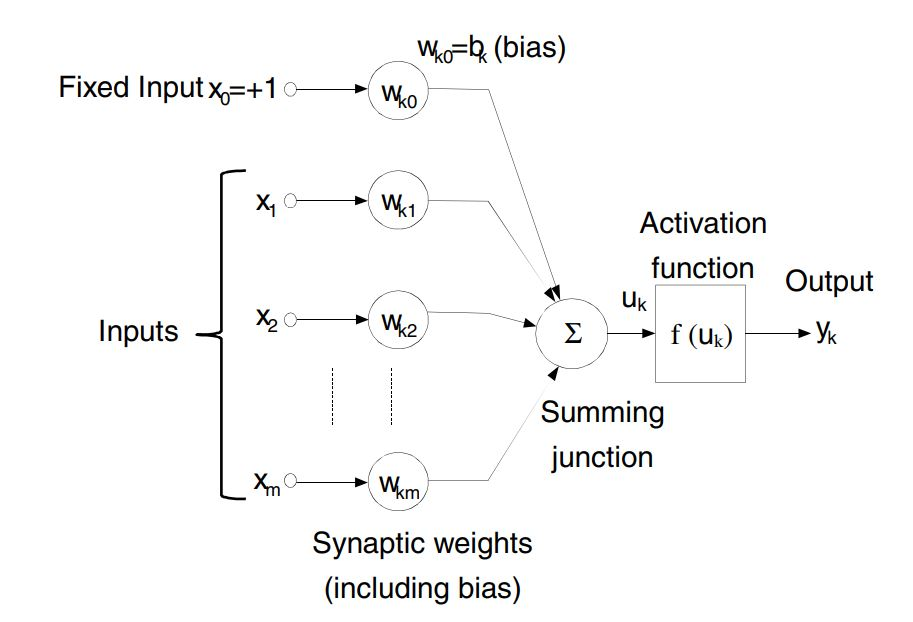
\includegraphics[width=\linewidth]{pictures/Perceptron.JPG} % leia abaixo
\caption{Modelo de um perceptron.}
\label{figura:Perceptron}
\end{figure}
	
	Para problemas mais complexos e que contenham grande quantidade de dados e características, pode-se criar uma rede de perceptrons em camadas como na ~\ref{figura:FeedforwardNN}, tal que a saída da primeira camada será a entrada para a próxima e as entradas, vieses e os pesos sejam definidos por cada camada, e não apenas para cada neurônio. As saídas de cada camada serão dados por 	
	$$ \textbf{y{\tiny j}} = f (\sum _{i} \textbf{x{\tiny i}} * \textbf{w{\tiny ij}} +  \textbf{b{\tiny j}}) $$
	Assim, uma rede de perceptrons multicamadas será uma função que mapeará os valores de entrada para valores de saída. E essa função dependerá dos valores de pesos e vieses da rede tal que diferentes valores e mesmas entradas fornecerão diferentes saídas. A rede poderá sempre ter a mesma arquitetura, mas terão valores diferentes de pesos e vieses para as variadas aplicações e domínios. \cite{Goodfellow-et-al-2016}
	
\begin{figure}[h]
\centering 
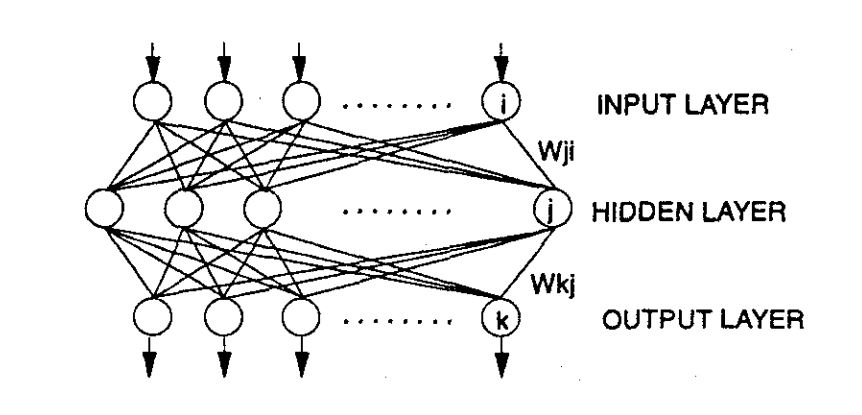
\includegraphics[width=10cm]{pictures/FeedForwardNN.JPG} % leia abaixo
\caption{Rede Neural Feedforward multicamadas.}
\label{figura:FeedforwardNN}
\end{figure}
 
	
	Um dos desafios é determinar quais serão os parâmetros, pesos e vieses ideais para a aplicação desejada. Para resolver esse problema, pode-se realizar um processo de treinamento, fornecer dados de entradas, propagar o sinal pela rede e posteriormente comparar as saídas da última camada com os valores de saída desejados através de um erro, e por fim utilizar um algorítimo de otimização para recalcular novos valores de parâmetros por toda a rede, como representado no diagrama da figura ~\ref{figura:NetTrain}. Esses processos são conhecidos como \textit{feedforward} e \textit{backpropagation}. \textit{Backpropagation} \cite{rumelhart1988learning} utiliza uma otimização do método do gradiente, um método de minimização para encontrar o mínimo local em um sistema iterativo, através do gradiente negativo para determinar o passo a ser tomado.	Para isso, deve-se recorrer ao cálculo diferencial, que permite determinar variações instantâneas. 
	
\begin{figure}[h]
\centering 
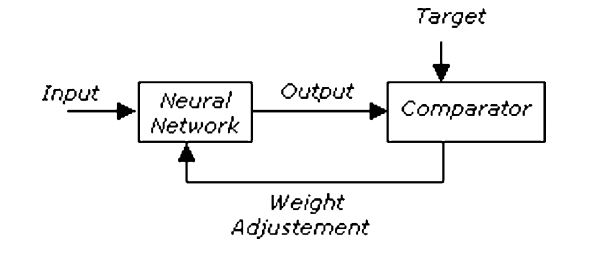
\includegraphics[width=10cm]{pictures/NetworkTrainer.JPG} % leia abaixo
\caption{Diagrama de blocos representante do treinamento supervisado de uma rede neural.}
\label{figura:NetTrain}
\end{figure}
 
	
	A atualização dos pesos de certa camada é dada por $$ \Delta \textbf{w{\tiny ij}} = - \alpha \frac{\partial C}{\partial \textbf{w{\tiny ij}}} $$ tal que $ \alpha $ é o passo, que determinará o quão rápido será a atualização, e $ \frac{\partial C}{\partial \textbf{w{\tiny ij}}} $ a derivada parcial da função custo em relação aos pesos da respectiva camada.
	
	Utilizando a regra da cadeia, tem-se que: $$ \frac{\partial C}{\partial \textbf{w{\tiny ij}}} = \frac{\partial C}{\partial f{\tiny j}} \frac{\partial f{\tiny j}}{\partial \textbf{w{\tiny ij}}}. $$ O primeiro termo é o erro que representa a variação da saída com o valor real esperado, dado por: $$ \delta{\tiny} = \frac{\partial C}{\partial f{\tiny j}}.$$	E o segundo termo pode ser simplificado por $$ \frac{\partial f{\tiny j}}{\partial  \textbf{w{\tiny ij}}} = \frac{\partial }{\partial  \textbf{w{\tiny ij}}} (\sum _{i} \textbf{x{\tiny i}} * \textbf{w{\tiny ij}} +  \textbf{b{\tiny j}}) =  \textbf{x{\tiny i}} $$
	
	Então pode-se escrever a derivada como: $$ \frac{\partial C}{\partial \textbf{w{\tiny ij}}} = \delta{\tiny} \textbf{x{\tiny i}} $$.
	
	É possível perceber que o algoritmo dependerá da função custo e da função de ativação escolhida e ambas devem ser diferenciáveis.
		
		\subsection{Redes Neurais Recorrentes (RNN)}
	
	Apesar da grande diversidade de aplicações possíveis com redes neurais, elas não conseguem aprender com eventos que ocorrem em uma sequência, tal que a ordem também seja importante. Com redes Feedforward, a propagação ocorre somente para um sentido, tal que a saída de uma camada se torna entrada da camada seguinte em uma rede de multicamada. Em redes neurais recorrentes (RNN, do inglês \textit{Recurrent Neural Networks}) \cite{elman1990finding} as saídas de uma camada podem se tornar entradas para a própria camada ou ainda para anteriores, formando laços que ligam novas informações com as do passado e permitem a criação de memória na rede. Assim como a memória em seres humanos, elas conseguem distinguir entre eventos que ocorreram no passado e como eles afetam o comportamento presente, através do reconhecimento de padrões em sequências de dados que adicionam uma dimensão temporal à rede e encontrando correlações em momentos distantes. Sua nova função de saída será dada por $$ y_{t} = f(W x_{i} + U y _{t-1}) $$ tal que $ U $ conterá informações referentes a recorrência da rede. 
	
	O treinamento é realizado através do Backpropagation Through Time (BPTT) \cite{werbos1990backpropagation}, uma variação do Backpropagation para redes Feedforward para as particularidades das redes RNN, mas ainda com o mesmo princípio de minimização da função de custo em relação aos pesos. Por outro lado, esse treinamento sofre um problema de dissipação do gradiente. \cite{sutskever2013training} \cite{bengio1994learning} Ao adicionar mais camadas ocultas na rede, o gradiente diminui a cada camada tal que ele passa a ser ínfimo e o treinamento praticamente para nas camadas iniciais. Assim, a rede passa a não reconhecer eventos muito distantes na sequência temporal. \cite{glorot2010understanding}
		
		\subsection{Long short term memory (LSTM)}
	
	Para superar o problema da dissipação do gradiente, \textit{Long-Short Term Memory} (LSTM)\cite{hochreiter1997long} \cite{gers1999learning} deixa de utilizar \textit{perceptrons} como blocos fundamentais da rede, mas passa a utilizar blocos de memória. Dentro de cada bloco existem múltiplas funções de ativação, como mostrado na figura ~\ref{figura:lstmCell}, e não mais somente uma como no \textit{perceptron}, tal que podem ativar ou não três portas. Tais portas (do inglês \textit{input}, \textit{output} e \textit{forget gates}) controlam o fluxo de informação, permitindo a leitura ou escrita da rede. Elas identificam a importância de cada informação e a permitem ou bloqueiam através da sua abertura ou fechamento. Tal arquitetura soluciona o problema da dissipação do gradiente durante o treinamento e tem apresentado resultados satisfatórios no reconhecimento de padrões em sequências longas. \cite{gers2001long} \cite{greff2017lstm} \cite{sutskever2014sequence}
	
	\begin{figure}[h]
\centering 
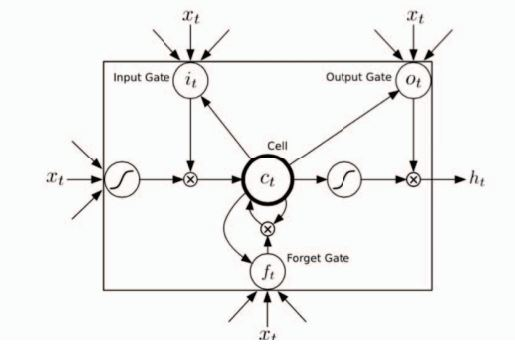
\includegraphics[width=10cm]{pictures/lstm.JPG} % leia abaixo
\caption{Arquitetura do bloco de memória de uma rede LSTM.}
\label{figura:lstmCell}
\end{figure}


% ------------> Na versão final, explicar melhor sobre o LSTM e incluir equações



	
\chapter{Metodologia}

\section{Tecnologias Utilizadas}

\subsection{Linguagem de programação}

	Existem hoje no mercado inúmeras linguagens de programação para a escolha e uso em diferentes aplicações, cada uma com suas vantagens e desvantagens sobre as outras para variados domínios. Dentro da comunidade científica tem-se utilizado vastamente da linguagem Python. É uma linguagem de programação interpretada, de alto nível, funcional, orientada a objetos e com semântica dinâmica criada na década de 1990 e com sua sintaxe semelhante a um pseudocódigo. 
	
	% ------> Referências
	
	Para aplicações que o foco principal não seja o desenvolvimento de um software complexo como para cientistas e engenheiros em prototipagem e testes, é interessante o uso de uma linguagem com uma curva de aprendizado rápida, fácil leitura, com sintaxe semelhante a linguagem natural, e manutenção e contendo menos linhas de código que em outras como Java ou C++. Ainda suporta módulos e pacotes de extensão, e novos pacotes podem ser criados para estender as suas funcionalidades. Por esse motivo, tem sido muito utilizada no meio científico, com pacotes específicos voltados a estrutura de dados, visualização, computação científica, entre outros. Tais características, presentes na linguagem python, fazem com que ela seja muito utilizada em meios científicos e acadêmicos. 
		
	Para o seu desenvolvimento, é possível utilizar diversas interfaces de programação e edição de texto. Jupyter é uma aplicação de internet interativa de um ambiente de programação com licença livre e código aberto. Um notebook é uma documento que combina execução de código, linguagem rica, fórmulas matemáticas, gráficos e media tal que facilita a leitura humana. O aplicativo permite sua execução em um navegador de internet, podendo ser local ou em um servidor remoto. A execução local fica restrita à capacidade computacional da máquina onde o código será interpretado, com quantidade muito limitado de memória RAM e poder de processamento. 
	
	% ------> Referências
	
	Modelos de redes neurais e em especial de deep learning, que requerem uma grande quantidade de dados para seres analisados, serão limitados em computadores pessoais e bibliotecas de programação convencionais, uma vez que todos os dados a serem analisados precisam estar guardados na memória da máquina para serem acessados em algum momento durante a execução. E ainda python não possui a mesma velocidade de execução de outras linguagens de baixo nível, como Java e C++, uma vez que é uma linguagem interpretada durante a execução, e não compilada.  Há então a necessidade de se buscarem outras alternativas para suprir tal necessidade. Uma biblioteca muito utilizada e escrita em C e como interface com python é Pandas, que é implementada e utilizada para manipulação e análise de grandes bases de dados de maneira otimizada. 
	
\subsection{Tensorflow}

	A criação de modelos de redes neurais é uma tarefa muito dispendiosa e de elevada complexidade, necessitando criar todas as conexões neurais e possíveis recursões de algumas redes. Uma forma de criar tais redes é através da utilização de tensores (vetores multidimensionais) como arestas de dados, tais quais fluem entre nós, que representam operações. Então uma aresta carrega informação de um nó para outro, e o resultado da operação se torna a entrada para outra. Esse tipo de programação já é implementada na biblioteca Tensorflow, que é gratuita, de código aberto criada e mantida pela Google, escrita em C++ e com suporte para diversas outras, tal como python. Foi criada e é utilizada para desenvolvimento de modelos de inteligência artificial e aprendizado de máquina. Um benefício desse tipo de programação é que as operações não precisam mais ser realizadas sequencialmente, mas podem ser paralelas. Dessa forma pode-se agendar as tarefas no processador de maneiras mais eficientes, distribuindo  melhor entre os recursos, como várias unidades de processamento em uma única máquina ou até mesmo em diferentes máquinas. 
	
	% ------> Referências
	
	Por outro lado, a criação dessa rede de grafos ainda pode ser muito complexa e não intuitiva. Pode-se utilizar uma ferramenta de interface entre os dois domínios. Keras é uma Interface de Programação de Aplicação (API, do inglês \textit{Application Programming Inferface}) de alto nível para desenvolvimento de redes neurais e escrita em python. Ela roda sobre outras bibliotecas de aprendizado de máquina, como Tensorflow, utilizando seus recursos como \textit{backend}. Foi criada com o objetivo de facilitar o desenvolvimento de modelos de rede neurais para experimentação, pesquisa e até produção, e para isso já possui implementado os modelos mais utilizados, como LSTM. Dentre seus benefícios estão a rápida prototipagem, sendo modulares e extensivas, suporte para redes neurais convolucionais e recorrentes e suporte a CPU e GPU.
	
	% ------> Referências

\subsection{Google Colaboratory - Colab}

%  Faltam referências ---------------------------
	Redes neurais têm uma grande necessidade de processamento paralelo entre os nós de cada camada, logo, para diminuir o tempo de treinamento, pode-se utilizar uma central de processamento com múltiplos núcleos que permita processamento paralelo. CPUs podem possuir múltiplos núcleos, mas reduzidos a algumas dezenas, já GPUs possuem microprocessadores capazes de operar em paralelo para realizar um elevado número de operações mais simples em um tempo muito mais baixo. O uso de GPUs é recomendado para a utilização de redes neurais artificiais, podendo realizar as muitas operações em paralelo, aumentando a performance. A Google, com o objetivo de incentivar a pesquisa e desenvolvimento de aplicativos de aprendizado de máquina, mantém uma plataforma online na nuvem, tal que desenvolvedores possam utilizar sua infraestrutura remotamente. Google Colaboratory, Colab, é uma implementação do aplicativo Jupyter Notebook que é executado na nuvem utilizando recursos computacionais fornecidos pela Google, tais como memória RAM, CPU e GPU, com otimização do consumo de recursos. Faz parte da plataforma de aplicativos de internet fornecidos pela empresa e permite que o notebook seja aberto e compartilhado pelo navegador de internet e ainda possui as bibliotecas mais utilizadas para desenvolvimento de aprendizado de máquina em python já instaladas e prontas para serem importadas. 
	
	% ------> Referências

% Falta Acabar ----------------------------------------
Tais ferramentas compõem arsenal no qual podem ser utilizadas em conjunto mantendo uma boa performance. Keras mantém a interface de fácil sintaxe em python para fácil criação de modelos de redes neurais com Tensorflow, mas não herda seu gargalo de baixa performance, uma vez que esse possui núcleo de alto desempenho escrito em C++. E ainda utilizando Google Colab e os seus recursos de processamento remoto com GPU, aumentam ainda mais a velocidade de processamento e treinamento das redes neurais testadas. 

\section{Base de dados}
	
	Novas tecnologias antes de serem adotadas são alvo de estudos para validação de seu funcionamento apropriado e econômico. Para determinar a viabilidade da utilização em grande escala de medidores inteligentes integrados na Irlanda, a CER realizou um grande ensaio em parceira com as concessionárias de distribuição de energia elétrica para sua instalação da infraestrutura necessária para seu funcionamento e com isso poder fazer estudos. Os dados gerados pelos medidores, com medições durante 1 ano e meio entre 2009 e 2011 e com frequência de 30 minutos foram disponibilizadas ao público para estudos e testes. 
	
	% ------> Referências
	
	Para se realizar análise de dados, é necessário uma etapa inicial de preparação e condicionamento dos dados a serem utilizados. Tal etapa vai desde a obtenção dos dados até a organização no formato correto para ser utilizado no modelo, passando por diversas outras etapas. A disciplina responsável é conhecida como Engenharia de Dados. Nesse trabalho, foram necessária diversas modificações na estrutura da base de dados. 
	
	A base de dados original é composta por três colunas. A identificação do medidor, a energia consumida durante o intervalo de 30 minutos de medição (em kWh) e um código de 5 dígitos representante das datas, como na tabela ~\ref{table:RawData} com os primeiro valores da base. Esse código era composto pelos 3 primeiros dígitos representando o dia do ano que a medida foi realizada (dia 1 é 1 de janeiro de 2009), e os 2 últimos dígitos o horário do dia (1 a 48 para cada 30 minutos, com 1 sendo 00:00:00 até 00:29:59). Cada um dos horários foram transformados em \textit{timestamps} sequenciais com horário e dia separadamente, como na tabela ~\ref{table:CleanData}. Uma base auxiliar é disponibilizada e contém o tipo de consumidor para cada identificador, dentre eles podiam ser residenciais, pequenos ou médios empreendimentos ou industriais. 
	
\begin{table}
\centering
 \begin{tabular}{|c|c|c|} 
 \hline
 Identificador & Timestamp & Medida \\ [0.5ex] 
 \hline\hline
  3533    &      19919&    0.6210\\
 \hline
  3533     &     19920 &   0.6760\\
 \hline
  3533     &     19921  &  0.9960\\
 \hline
  3533     &     19922   & 2.2440\\
 \hline
  3533      &    19923   & 3.9170\\
 \hline
  3533       &   19924&    2.1740\\
 \hline
\end{tabular}
\caption{Exemplos de linhas da base de dados original.}
\label{table:RawData}
\end{table}


\begin{table}
\centering
 \begin{tabular}{|c|c|c|} 
 \hline
 Identificador & Timestamp & Medida \\ [0.5ex] 
 \hline\hline
  3533    &      2015-07-19  09:30:00&    0.6210\\
 \hline
  3533     &     2015-07-19 10:00:00&   0.6760\\
 \hline
  3533     &     2015-07-19  10:30:00&  0.9960\\
 \hline
  3533     &     2015-07-19 11:00:00    & 2.2440\\
 \hline
  3533      &    2015-07-19  11:30:00  & 3.9170\\
 \hline
  3533       &   2015-07-19 12:00:00&    2.1740\\
 \hline
\end{tabular}
\caption{Exemplos de linhas da base de dados com datas no formato correto}
\label{table:CleanData}
\end{table}
		
	Na etapa de limpeza dos dados, são removidos outliers, dados de medidas com mais de 5 desvios padrão; e dados duplicados, com mesmo timestamp e identificador. São também identificados timestamps faltantes, que não contenham nenhuma medição para determinado dia e horário. Como para sequências temporais é necessário que se mantenha o igual intervalo temporal entre as medidas, os dados precisam ser preenchidos, e para manter a simplicidade e pelo tamanho da base de dados, será preenchido com interpolação para todos os identificadores com dados nos timestamps anteriores e posteriores. São identificados também campos com valores nulos, que caso sejam valores isolados, pode-se interpolar com valores anteriores e posteriores, ou para grandes sequências, uma vez que se tem grande quantidade de medidores, remover todos os dados desse medidor. 
	
	Realizar tais procedimentos em bases de dados de dimensões muito elevadas é um desafio, uma vez que ela precisa ficar armazenada na memória da máquina ou ser realizada em múltiplas partes menores e os resultados serem agregados ao final. E ainda para o processamento, que pode ser muito demorado e levar vários minutos ou até horas para ser completado. Para esses problemas, é utilizada a ferramenta Pandas, uma biblioteca escrita em C e com interface para python, com o objetivo de auxiliar a preparação de dados e otimizada para grandes estruturas de dados. Fornece funções já implementadas, removendo a necessidade de utilizar linguagens de domínio específico. Pode ser utilizado também o Colab, tal que toda a infraestrutura disponibilizada na nuvem permitiu a realização da preparação com blocos maiores de dados, com maiores recursos que seriam disponíveis em máquinas locais. E ainda deixam as máquinas locais livres para o desenvolvedor desempenhar outras tarefas. 
	
	% -------> Na versão final, descrever detalhadamente a metodologia (Explicar, fluxograma, etc - CRISP
	
%	Determinar relação entre tipo de consumidor e seus comportamentos e padrões de consumo
%	Determinar diferentes estratégias de operação para diferentes tipos de consumidores
%	Consumidores tem padrões diferentes por possuírem e utilizarem equipamentos diferentes
%	Exemplos de diferentes consumidores nesse paper
%	Curva de carga de um consumidor específico muito diferente da curva agregada do sistema \cite{li2016short}

%	Diferentes perfis de consumo na base de dados da Irlanda
%	Dependendo da renda, estação do ano e horário do dia
%	Dados foram agregados com soma de todos eles
%	\cite{viegas2015electricity}


\chapter{Análise experimental}
% ----------------------------------------------------------
% Finaliza a parte no bookmark do PDF
% para que se inicie o bookmark na raiz
% e adiciona espaço de parte no Sumário
% ----------------------------------------------------------

	Os experimentos serão realizado com diferentes arquiteturas de redes LSTM, variando-se a quantidade de camadas, e seus parâmetros de treinamento como o passo. Pode-se também verificar a diferença entre o treinamento com cargas residenciais e de pequenas e médias empresas separadamente ou juntas, observando como será o resultado. Os resultados finais serão avaliados pelos desvio quadrático médio (RMSE, do inglês \textit{Root Mean Square Error}), entre o valor de saída da rede após o treinamento, de uma base de dados de teste, e o valor esperado, fornecido por essa base de dados. 
	
	% ------> Na versão final , apresentar e explicar os resultados	
	
\phantompart

% ---
% Conclusão
% ---
\chapter{Conclusão}
% ---

	O monitoramento e controle da rede de distribuição de energia elétrica é de grande necessidade para as concessionárias para auxiliar na operação do sistema mantendo-o seus valores operativos dentro de faixas limites aceitáveis.
	Previsão de carga de curto prazo auxilia esse controle, mas a previsão de cargas individuas de todo o sistema no contexto de redes inteligentes é dificultada por técnicas já utilizadas pelo seu grande volume de dados. 
	
	Aprendizagem profunda auxilia esse problema, uma vez que é capaz de analisar grande quantidades de dados, através de modelos de baixa complexidade sem dados físicos do domínio, mas somente através de dados sequenciais passados para seu treinamento. LSTM pode ser uma solução uma vez que consegue manter em sua rede conhecimento de curto e longo prazo. 
	
	
	% ------> Conclusões parciais e trabalhos futuros
	
	
% ----------------------------------------------------------
% ELEMENTOS PÓS-TEXTUAIS
% ----------------------------------------------------------
\postextual
% ----------------------------------------------------------

% ----------------------------------------------------------
% Referências bibliográficas
% ----------------------------------------------------------
\bibliography{abntex2-modelo-references}

% ----------------------------------------------------------
% Glossário
% ----------------------------------------------------------
%
% Consulte o manual da classe abntex2 para orientações sobre o glossário.
%
%\glossary

% ----------------------------------------------------------
% Apêndices
% ----------------------------------------------------------

% ---
% Inicia os apêndices
%% ---
%\begin{apendicesenv}
%
%% Imprime uma página indicando o início dos apêndices
%\partapendices
%
%% ----------------------------------------------------------
%\chapter{Quisque libero justo}
%% ----------------------------------------------------------
%
%\lipsum[50]
%
%% ----------------------------------------------------------
%\chapter{Nullam elementum urna vel imperdiet sodales elit ipsum pharetra ligula
%ac pretium ante justo a nulla curabitur tristique arcu eu metus}
%% ----------------------------------------------------------
%\lipsum[55-57]
%
%\end{apendicesenv}
% ---


% ----------------------------------------------------------
% Anexos
% ----------------------------------------------------------

% ---
% Inicia os anexos
%% ---
%\begin{anexosenv}
%
%% Imprime uma página indicando o início dos anexos
%\partanexos
%
%% ---
%\chapter{Morbi ultrices rutrum lorem.}
%% ---
%\lipsum[30]
%
%% ---
%\chapter{Cras non urna sed feugiat cum sociis natoque penatibus et magnis dis
%parturient montes nascetur ridiculus mus}
%% ---
%
%\lipsum[31]
%
%% ---
%\chapter{Fusce facilisis lacinia dui}
%% ---
%
%\lipsum[32]
%
%\end{anexosenv}

%---------------------------------------------------------------------
% INDICE REMISSIVO
%---------------------------------------------------------------------
\phantompart
\printindex
%---------------------------------------------------------------------

\end{document}
